\documentclass[12pt]{article}

\usepackage[utf8]{inputenc}
\usepackage{ngerman}

\usepackage{graphicx}
\usepackage{subfigure}

\usepackage{lipsum}
\usepackage{pdfpages}

\usepackage{color}
\usepackage{verbatim}
\usepackage{float}

\usepackage{varioref}
	\labelformat{figure}{Abbildung~#1}


\begin{document}
%opening

%\includepdf{Titlepage}

\newpage

\tableofcontents

\newpage
	
\section{Einleitung}

\vspace{2cm}
\subsection{Spielprinzip}

\vspace{2cm}
\subsection{Zielsetzung}

\vspace{2cm}
\subsection{Projektumfeld}
- erfahrungen, background
 grund


\newpage
\section{Projektplanung}

In diesem Abschnitt werden die Ergebnisse der ersten Planungen festgehalten, wie wir das Projekt umsetzen wollen. Hierbei sind besonders wichtig, für welche Prozesse und Workflows wir uns entschieden haben. \newline
Da wir am Anfang und selbst erstmal im Team finden musste, um unsere Stärken und Spezialisierungen kennenzulernen und uns nicht sicher waren, wieviel wir wirklich umsetzen können, haben wir uns für agiles Projektmanagement entschieden. Dabei werden in kurzen Phasen sogenannte Sprints durchgeführt, in denen immer fest definierte Teilaufgaben erledigt werden. Die Besonderheit bei einem Sprint ist, das am Ende eines Sprints immer eine funktionsfähiges Programm stehen muss, ohne offene, unvollständigen Klassen. \newline
Als unterstützendes Tool wurde der integrierte Kanban von GitHub benutzt. Wir definierten uns relativ viele eigene Label, um den Informationsgehalt der einzelnen Tasks noch zu verstärken.
So entwickelte sich unser Kanban relativ schnell zum zentralen Anlaufpunkt. Wir hatten stets tagesaktuelle Informationen über die Fortschritte der anderen Teammitglieder:
\begin{itemize}
	\item alle Tasks in ihrem aktuellen Bearbeitungsstatus, anhand der zugeordneten Spalte im Kanban
	\item Art und Ausprägung der Aufgaben, anhand farblich markierter Labels
	\item neue Probleme, Rückfragen oder Bugs waren durch eindeutige Farben direkt erkennbar.
	\item bearbeitete Tasks, welche zur Überprüfung bereit sind, sind in einer eigenen Spalte aufgelistet
\end{itemize}
Grundsätzlich bestand der Workflow darin aktuell wichtige Tasks, die für den nächsten Meilenstein wichtig sind in die Spalte \glqq Pipeline\grqq{} zu ziehen. Sobald sich einer von uns einer Anforderung angenommen hat, so hat er diese in den Status \glqq in Bearbeitung\grqq{} verschoben. Nach Bearbeitung einer Aufgabe wurde diese dann zur \glqq Review\grqq{} überführt. Sobald ein anderes Teammitglied Tasks aus der \glqq Review\grqq{} überprüft hat, wurden sie entweder archiviert oder in die Spalte \glqq Probeleme\grqq{} gesteckt. Der Status \glqq Probleme\grqq{} war außerdem Sammelstelle für Bugs oder wenn jemand dringend Unterstützung benötigt und in seinem aktuellem Task nicht weiterkommt.

\vspace{2cm}
\subsection{Projektphasen}
Wir haben unsere verfügbare Zeit in drei Phasen aufgeteilt, um mit realistischen Erwartungen und Ergebnissen arbeiten zu können. \newline
\subsubsection{Lernphase}
Wir haben die ersten beiden Meilensteine als Lern- und Findungsphase definiert. Dabei haben wir uns bewusst dafür entschieden unsere Aufgabenpakete und Ziele gering zu halten.
Denn für uns war es wichtig, dass wir in den ersten Wochen hauptsächlich lernen mit dem Framework und allgemein der 3D-Spieleprogrammierung um zugehen. Ein zusätzlicher Erfolg war, dass wir relativ gut lernten, wie wir uns gegenseitig unterstützen konnten. In dieser Phase haben wir dann auch einen gemeinsamen Programmierstil und geeignete Coding-Coventions festgehalten. In dieser Phase haben wir unsere Grundlegende Struktur auch bewusst etwas aufwendiger implementiert, um es in den späteren, hektischeren Phasen leichter zu haben.

\subsubsection{Hauptphase}
Nach dem wir uns im Team gut eingespielt hatten, konnten wir den 3. und 4. Meilenstein relativ gut und ohne viel Stress bewältigen. Wir hatten unsere regelmäßigen Treffen zur Abstimmung und jeder hat für sich seine wöchentlichen Aufgaben eingeteilt und abgearbeitet. \newline
In dieser Phase wurde aber auch relativ viel am GameDesign und an der Meilensteinplanung geändert, da viele Details und Besonderheiten sich erst herausstellen, wenn man am Objekt selber arbeitet. So haben sich einige Aufgaben zwischen den Meilensteinen verschoben oder wurden getauscht. Dies hatte oft den Grund, dass für die aktuelle Funktionalität gewisse Implemntierungen und Features Vorrang hatten. Hierbei spielte auch manchmal eine gewisse Abhängigkeit unter den einzelnen Teammitgliedern eine Rolle.

\subsubsection{Schlussspurt}
Uns war von Anfang an klar, dass es in den letzten 2-3 Wochen vor der Abgabe nochmal eine etwas stressigere Phase geben wird, in der nochmal versucht wird alle möglichen Features einzubauen, die noch fehlen, das Spiel Rund zu machen, kleinere Bugs die ignoriert wurden zu beheben. Um ein stimmiges Endresultat abliefern zu können, haben wir uns auch selbstständig diese Wochen so eingeplant, dass wir dort die Kapazitäten haben einen kleinen Schlussspurt hinzulegen, um unsere selbst gesteckten Ziele zu erreichen.


\vspace{2cm}
\subsection{Ressourcenplanung}
Für die Umsetzung des Projektes ist es notwendig im Voraus alle nötigen Ressourcen zu definieren und zu verteilen. Hierbei spielen sowohl personelle und materielle Ressourcen eine Rolle, als auch die Planung von nötiger Software oder Fremd-Bibliotheken. \newline
\subsubsection{Ressource Mensch}
Hier haben wir uns einfach an unsere Fähigkeiten und Neigungen gehalten, sodass sich relativ schnell herauskristallisiert hat, wer welche Rollen und Aufgaben übernimmt. So hat Alex die Hauptführung über den Bereich des 3D-Modellings übernommen und hat die meisten Modelle und Texturen für die Modelle übernommen.
Da es aber auch eine Vorgabe war, dass jeder im Team seinen Anteil an der Programmierung leistet, hat Alex sich dazu bereit erklärt das Menü-System zu implementieren. \newline
Lars hat großteile der Programmierung übernommen, seine Aufgaben lagen vorallem in der Umsetzung der 3D-Optik, Kamera und Einbinden der Animationen, sowie einige Kern-Features, wie z.B. Collision oder das Soundsystem. \newline
Das Projektmanagement hat größtenteils Christoph übernommen. Programmiertechnisch hat er bei einem Großteil der Spielrelevanten Features mitgearbeitet und dafür gesorgt, dass die einzelnen Systeme miteinander agieren können. Zusätzlich liegt alles was mit 2D-Art zu tun hat in seinem Aufgabenbereich. Neben vielen Grafiken für Menü oder UI zählt hier auch das Paritkelsystem dazu.

\subsubsection{Ressource Software}
Wir haben für das gesamte Projekt auf Software zurück gegriffen, die entweder kostenlos zur Verfügung steht, oder die bereit in unserem Besitz ist und daher für dieses Projekt ohne Entstehung von Kosten mit genutzt werden konnten.\newline
Um gleichzeitig ohne viel Konflikte am gleichen Projekt arbeiten zu können, ist es wichtig, dass man sich auf eine gemeinsame Software - vor Allem mit gleicher Version - entscheidet. \newline
Als Framework für unser Spiel wählten wir MonoGame 3.5, damit war auch die Programmiersprache C\# größtenteils schon vorgegeben. Als IDE nutzen wir Visual Studio mit den Standards aus der 2015 Version.
Dadurch konnten wir Kompatibilitätsprobleme zwischen verschiedenen C\# Versionen vorbeugen, da wir uns auf einen gemeinsamen Standard einigten.
Wir haben uns dazu entschieden die Animation mit Hilfe einer Fremdem Bibliothek umzusetzen. \newline
Als Software für 3D-Modelierung wurden hauptsächlich Solid Edge und Blender benutzt. Texturen und andere 2D-Elemente wurden größtenteils mit PhotoShop angefertigt und bearbeitet.
Eine detailliertere Auflistung der gesamten Software ist Tabelle \ref{tbl:software} zu entnehmen.
\begin{table}[H]
\centering
	\begin{tabular}{p{0.5cm}p{9cm}}
		\textbf{ }  & \textbf{Name der Software/ des Services} \\
		\hline
		\textit{1}          & \textnormal{Visual Studio 2015 Enterprise}            \\
		\textit{2}          & \textnormal{Visual Studio 2017 Community}            \\
		\textit{3}          & \textnormal{Blender 2.78}            \\
		\textit{4}          & \textnormal{Solid Edge ST9}            \\
		\textit{5}          & \textnormal{PhotoShop CS5}            \\
		\textit{6}          & \textnormal{Audacity 2.1.3}            \\
		\textit{9}          & \textnormal{Git 2.7}  \\
		\textit{10}          & \textnormal{Turtoise Git 2.4}            \\
		\textit{11}          & \textnormal{TeXstudio 2.11 + MikTex}       \\
		\textit{12}          & \textnormal{GoogleDocs + Google Präsentationen)}  \\
		\textit{13}          & \textnormal{GitHub}  \\
		\hline
	\end{tabular}
	\caption{Auflistung verwendeter Software und Services}	
	\label{tbl:software}	
\end{table}

\subsubsection{Ressource Assets}
Für Assets haben wir versucht alles so gut wie möglich komplett selber zu erstellen. Einzelheiten zu den verschiedenen Assets sind dem entsprechenden Abschnitt zu entnehmen.
Die einzige Ausnahme bilden hier einige wenige Sounds die wir von Plattformen genommen haben, die Sounds mit CreativeCommons - Lizenz anbieten. 

\vspace{2cm}
\subsection{Entwicklungsprozess}
Um den Entwicklungsprozess mit dem agilen Verfahren umzusetzen, ist es nötig sich einen gewissen regelmäßigen Ablauf einzuplanen. \newline
Wir haben uns dazu entschieden ein wöchentliches Planungstreffen abzuhalten,
in dem wir den aktuellen Fortschritt auswerten und die weiteren Tasks und Meilensteine einplanen. Dieses Treffen gab uns vor allem auch die Zeit und den Raum über Probleme oder eventuelle Verschiebungen zu reden. So konnten wir relativ gut auf Planänderungen agieren und unsere jeweilige Wochenaufgaben neu einplanen. \newline
Zusätzlich haben sich die Hauptprogrammierer einmal wöchentlich gemeinsam getroffen, um sich auch gegenseitig aushelfen zu können und auch mal mit einem Augenpaar mehr auf gewisse Entscheidungen in der Umsetzung blicken zu können.
Die sonstige Zeiteinteilung wurde den Teammitgliedern zur eigenen Verantwortung freigestellt. Dies hat sehr gut funktioniert. Wohl auch durch die wöchentlichen Planungstreffen, in denen man Bericht ablegen muss, über seine Fortschritte der letzten Woche.

\newpage
\section{Das Spiel}

\vspace{2cm}
\subsection{Hauptmenü \textcolor{blue}{(QA - Lars )}}

Das Hauptmenü stellt den Einstieg in unser Spiel dar. Hier wird der Spieler empfangen.

\vspace{1cm}
\subsubsection{Spiel Starten \textcolor{blue}{(QA - Lars )}}

Durch das Betätigen des Buttons „Starten“ gelangt man in den Ingame-Bereich. Bevor es mit dem Spielen losgeht, öffnet sich am Anfang jedes
Levels ein kleiner Tutorialbildschirm, welcher auch als Pause für den Spieler gedacht ist. Weiterhin kann er hier kurz verweilen um sich vorzubereiten
und so die Konzentration zu steigern.

\vspace{1cm}
\subsubsection{Einstellungen \textcolor{blue}{(QA - Lars )}}

Mit den Settings kann man seine persönlichen Einstellungen an dem Spiel vornehmen. Es lassen sich der Schwierigkeitsgrad und die Musiklautstärke
ändern. Auch gibt es hier eine ausführliche Beschreibung der Steuerung.

\vspace{1cm}
\subsubsection{Statistiken \textcolor{blue}{(QA - Lars )}}

Unter Statistics lässt sich der Spielfortschritt in den einzelnen Leveln begutachten. So findet man eine detaillierte Auflistung von Timeboni, eingesammelten
Münzen und den Score für jedes Level. Des Weiteren werden auch die gesamte Todeszahl und der Totalscore erfasst. Nach Beenden des Spiels wird die Statistik gelöscht. Die Statistik wird zu dem  nur zu einem Run aufgestellt, sobald der Spieler das Spiel durchgespielt hat und einen neuen Run startet wird die alte Statistik gelöscht.

\begin{figure}
	\centering
	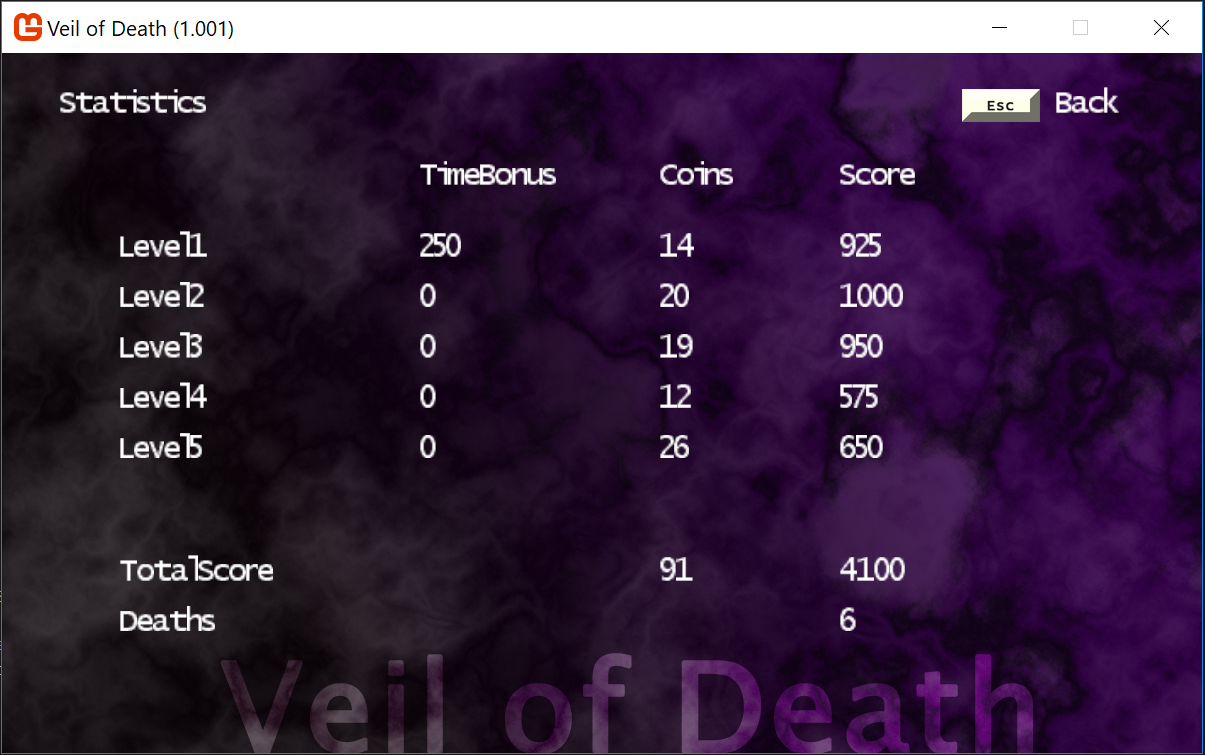
\includegraphics[width=1\textwidth]{Statistics}
	\caption{Statistik
		\label{fig:statistics}}
\end{figure}

\vspace{1cm}
\subsubsection{Credits \textcolor{blue}{(QA - Lars )}}

Diese Option gibt Auskunft über die Konstellation des Teams und die jeweiligen Aufgabenbereiche.

\vspace{1cm}
\subsubsection{Sonstiges}

\vspace{2cm}
\subsection{Spielwelt}

\vspace{1cm}
\subsubsection{Levelgenerator}
Zur Generierung der einzelnen Level wollten wir ein System implementieren, welches uns ermöglicht relativ einfach jederzeit Level zu ändern und neue Level hinzuzufügen, ohne großartig im Code was ändern zu müssen.
Wir haben einen Levelgenerator geschaffen, der die Welt anhand von Bitmap-Dateien aufbaut. Die Bitmap-Datei dient dabei quasi als Skizze für das resultierende Level. Jeder Pixel der Grafik stellt ein Block im Spiel dar.
Es wurde ein Kodierung definiert, die angibt welche Farbe für welches Objekt im Spiel steht. Mit diesem Wissen kann nahezu Jeder mit Hilfe von einfachsten Bildbearbeitungsprogrammen wie Paint seine eigenen Maps zeichnen. \newline
Im Code selber liest der Generator die Farbwerte aus und schlägt in einem Dictionary nach, welches Model auf der aktuellen Position geladen werden soll.
Eine Besonderheit hier ist, dass das Dictionary je nach Art des Levels andere Modelle, bzw. andere Texturen für die Modelle lädt. So können wir optisch unterschiedliche Welten generieren, die trotzdem auf den gleichen Regeln in der Bitmap-Datei beruhen.

\vspace{1cm}
\subsubsection{Player}

\vspace{1cm}
\subsubsection{Fallen \textcolor{blue}{(QA - Lars )}}

In unserem Spiel finden zwei Arten von Fallen Verwendung. Es gibt Fallen, die den Spieler verlangsamen. Weiterhin haben wir eine
weitere Art Fallen, die zum plötzlichen Tod führen. Dieser wird durch die Kollision mit den Fallen ausgelöst. Der Tod wird durch die
Spiketrap und die Spikeroll verursacht. Außerdem ist zu erwähnen, dass die Spikeroll beweglich ist. Je nach Schwierigkeitsgrad nimmt
die Bewegungsgeschwindigkeit dieser zu. Bei der Slowtrap wird der Spieler für eine bestimmte Dauer verlangsamt. Nach dem der Spieler
mehrere Male durch die Slowtrap gelaufen ist, wird er letztendlich vom Veil eingeholt und stirbt. Dadurch haben wir verschiedene Faktoren,
die das Spiel zusätzlich erschweren sollen.

\vspace{1cm}
\subsubsection{Feedback}

\vspace{1cm}
\subsubsection{Assets}

\newpage
\section{Technische Umsetzung}

\vspace{2cm}
\subsection{Codestruktur}
\textcolor{green}{- siehe TDD}

\vspace{1cm}
\subsubsection{GameStates}
\textcolor{green}{- alle mal kurz anreißen}

\vspace{1cm}
\subsubsection{Globale Klassen \textcolor{blue}{(QA - Lars )}}
%\textcolor{green}{- GameConstants \newline
%- Gamemanager (siehe TDD)}

In der GameConstants-Klasse wurden alle static-Objekte des Projektes angelegt. Hier zu gehören Variablen die klassenübergreifend gebraucht werden.
Weiterhin sind hier alle wichtigen Soundeffekte hinterlegt. Eine Kamerainstanz ist auch hinterlegt. Des Weiteren sind auch wichtige Angaben zum Sprung
hier hinterlegt, wie die Sprungweite und Sprunghöhe. Der Vorteil dieser Klasse ist, dass hier alle Zahlenwerte gebündelt gesammelt wurden, die global im
Projekt verwendet werden. Dadurch sind Änderungen sehr schnell vornehmbar.

Der GameManager ist ein Singelton-Pattern in dem das Spiels verwaltet wird und bildet somit das Herz des Spiels. Durch unsere Mapgeneration auf die wir
vorhin eingegangen sind, ist es notwendig zu wissen, welche Fallen aktiv sind und welche nicht. Dafür werden die Fallen in ihren Listen gespeichert, welche
immer aktualisiert werden, durch hinzufügen oder löschen der Fallen. So gibt es für jede Fallenart eine Liste. Das gleiche Prinzip gilt auch für die Münzen.
Der Todesschleier wird von hier aus gesteuert. Levelverwaltung, Scorehandhabung und das Speichern der Statistik sind ein weiterer Bestandteil des GameManagers.

\vspace{2cm}
\subsection{InGame}

\vspace{1cm}
\subsubsection{Movement \textcolor{blue}{(QA/ Grafik fehlt - Lars )}}
%\textcolor{green}{- Lane prinzip \newline
%- Jump-Funktion (Parabel anhand von Geschwindigkeit)}

Unser Spielercharakter kann sich auf drei Arten fortbewegen. Er kann Rennen, Sliden und Springen. Der Sprung wurde an eine
Wurfparabel angepasst, sodass sich der Sprung wie ein Wurf verhält. Der Spielercharakter gewinnt an Höhe bis er den Scheitelpunkt
erreicht und sinkt danach wieder zu Boden. Dadurch ist der Sprung symmetrisch, sowohl die Anstiegs- und Abstiegskurve sind gleich.

%Grafik Wurfparabel einfügen

Durch das Laneprinzip unseres Spiels haben wir uns gegen einen flüssigen Übergang des Spielercharakters beim Wechseln der Lanes
entschieden. Wir lassen ihn wirklich zwischen den Lanes switchen, so dass er sich nicht in Zwischenbereichen aufhalten kann.

\vspace{1cm}
\subsubsection{Collision \textcolor{blue}{(QA - Lars )}}

\begin{comment}
\textcolor{green}{2 Arten: \newline
- AABB für Spiketrap und spikeroll \newline
- Gridposition für Coins und Slowtrap}
\end{comment}

In unserem Spiel haben wir zwei unterschiedliche Kollisionmethoden verwendet.
Zum Einen Arbeiten wir mit Gridpositions für statische Objekte und mit den
Axis-Alligned-Bounding-Boxes für bewegbare Objekte.\newline
\newline
Gridpositions eignen sich hervorragend für statische Objekte in Spielen, daher werden die Kollisionen
von Münzen und Slowtraps von ihnen verwaltet. Hier für werden die Positionen von unseren kollidirbaren
Objekten abgespeichert. Die Kollision wird dann mit Hilfe von if-Bedingungen berechnet.\newline
\newline
Axis-Alligned-Bounding-Boxes berechnen für uns die Kollisionen mit beweglichen Obejkten, so dass jedes Objekt seine eigene
Bounding Box hat. Hier für wird um das Objekt eine Hülle gespannt. In unserem Spiel haben wir die jeweiligen Maximalwerte
der Modelle in Betrachtung der Achsen gewählt. Die Kollision entsteht wenn die Minimalwerte der Achsen von Körper A kleiner
als die Maximalwerte von Körper B sind. Sowie die Maximalwerte der Achsen von Körper A größer sind als die Minimalwerte der
Achsen von Körper B. Anders gesagt wenn die erweiterte konvexe Hülle des einen Körpers, die des Anderen schneidet.

%Grafik einfügen



\vspace{1cm}
\subsubsection{Sontiges}

\vspace{2cm}
\subsection{GUI}
Die GUI dient dem Spieler als Interatkions- und Feedbackebene. Hier können ein großteil von Informationen auf sehr einfachem Weg bereit gestellt werden, welche dem Spieler über das aktuelle Spielgeschehen in Kenntnis setzen.
Wir haben uns dafür entschieden unsere GUI relativ schlank zu halten, um den Spieler nicht zu sehr von dem herausfordernden Hauptspiel abzulenken.
Eine wichtigen Hinweis, welchen wir den Spieler via GUI mitteilen ist seine Aktuelle Entfernung zum Ziel und sein Vorsprung zum gefährlichen Schleier des Todes. Beide sind als Icons auf einer Strecke dargestellt, die der Länge des Levels entspricht. \newline
Ein weiteres Element, welches wir über die GUI darstellen ist der Schleier selbst. Unterschreitet der Abstand des Spielers zum Schleier einen gewissen Schwellenwert, so wird der Spieler bereits von dessen Macht beeinflusst und sein Sichtfeld schränkt sich ein. Die Einschränkung des Sichtfeldes hat verschiedene Stufen, die abhängig von der Nähe der tödlichen Wolke sind.

\vspace{1cm}
\subsubsection{Panel System}
Für die Umsetzung der verschiedenen GUI-Elemente haben wir uns dafür entschieden ein eigenes Panel System zu implementieren, um das Erstellen von GUI-Masken oder weiteren Menüs einfacher wird.
Hierzu wird als erstes ein Basis-Panel erstellt, welches mit oder ohne Hintergrundgrafik geladen werden kann. Dieses Panel kann mit einer relativen oder festen Position in die Spielumgebung eingebaut werden.
Nun kann man beliebig viele Unterelemente zu dem Hauptpanel hinzufügen.
Dabei gibt es entweder die Möglichkeit ein Sprite (bzw. Grafik) hinzuzufügen oder einfach nur einen Text. Die Positionen dieser Elemente werden stets relativ zum Hauptpanel interpretiert. Wenn nun das Hauptpanel geändert wird, verhält es sich wie ein Anker zu all seinen Unterelementen, die sich wieder in richtiger Anordnung ausrichten.
Mehr als das hinzufügen der Elemente ist nicht nötig. Das Zeichnen übernimmt das Hauptpanel. Trotzdem ist es möglich die einzelnen Elemente anzusprechen und zur Laufzeit zu verändern (z.B. Hervorhebung der aktuellen Auswahl).

\vspace{2cm}
\subsection{Rendering}

\vspace{1cm}
\subsubsection{Aufbau}

\vspace{1cm}
\subsubsection{Weltkoordinaten \textcolor{blue}{(QA - Lars )}}

Der Up-Vektor in unserem Spiel ist nicht wie üblich die y-Achse sondern die z-Achse. Weiterhin bildet der Koordinatenursprung am 
Anfang nicht die Mitte unserer Lanes, er liegt am linken Rand. Darauf aufbauend wird die Spielwelt mit Hilfe unserer Blocksize generiert. Hierfür 
werden lediglich die x- und y-Achse benötigt. Die z-Achse wird für die Kollisionsberechnung benötigt. Die Kamera befindet sich am Anfang 
vor unserer eigentlich Spielwelt, um die gewünschte Perspektive zu erzeugen. Im weiteren Verlauf des Spiels verfolgt sie dann den Spieler
auf einer Linie entlang der y-Achse mit konstanter Geschwindigkeit. Die Kamera wurde somit aus dem Koordinatenursprung zu ihrem letztendlichen
Platz verschoben. Somit bildet die Weltmatrix diese Translation ab. Eine genaue Darstellung können sie \ref{fig:coordinates} entnehmen.

\begin{figure}
	\centering
	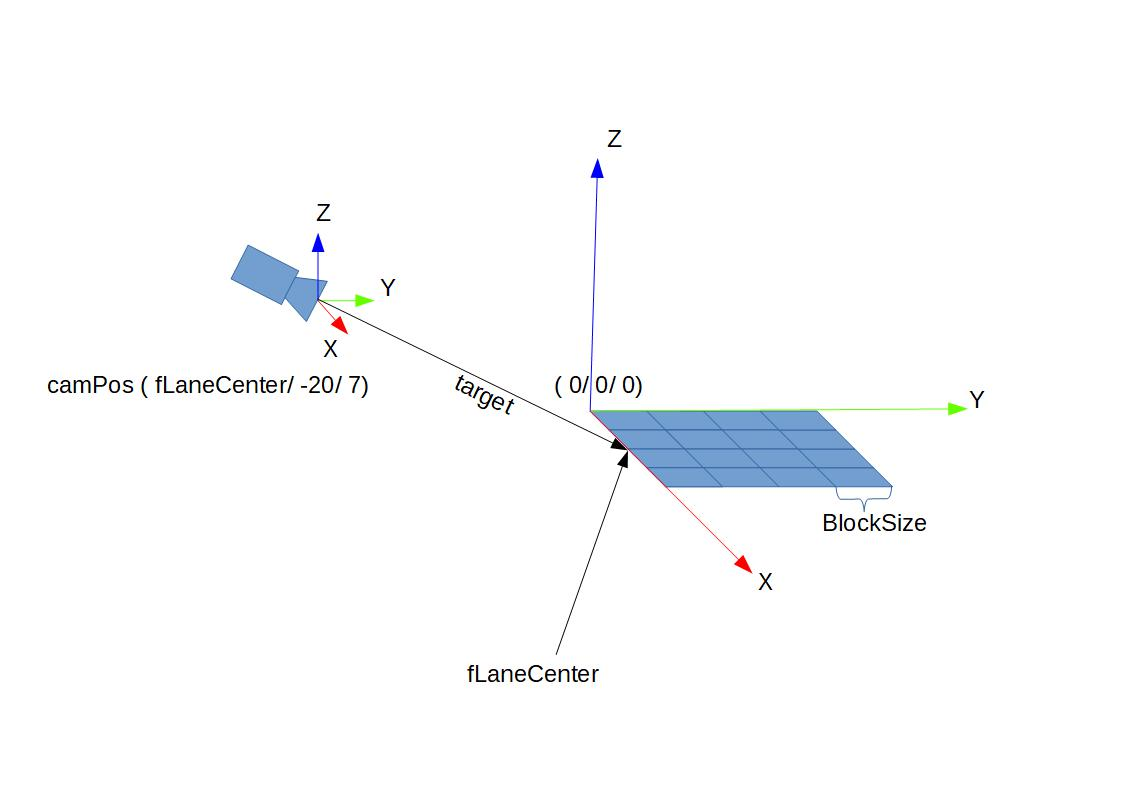
\includegraphics[width=1\textwidth]{Weltkoordinaten}
	\caption{Weltkoordinaten
		\label{fig:coordinates}}
\end{figure}

\vspace{1cm}
\subsubsection{Animation \textcolor{blue}{(QA - Lars )}}
Die Animation der Modelle erfolgt unter den Gebrauch einer Bibliothek. Hierfür benötigt man eine .x-Datei.
Des Weiteren wird eine Textdatei benötigt, in der festgehalten ist, wie das Modell animiert werden soll.
In dieser Textdatei kann man auf das jeweilige Modell bezogen so viele Methoden (Animationparts) erstellen
wie man möchte. Man kann entscheiden, ob die Animation wiederholt werden soll oder einfach gespielt wird.
Außerdem wird hier das Start- und Endframe der Animation festgelegt. Auch die Animationsdauer ist eine weitere
Einstellungsoption. Nach dem man die jeweiligen Einstellungen für seine Methoden festgelegt hat, kann man diese
im späteren Code unter ihrem angegebenen Namen aufrufen. Bevor man diese jedoch aufrufen kann, muss die
Textdatei gelesen werden. Es gilt weiterhin zu beachten, dass nur eine Animations gleichzeitig abgespielt werden kann.
Darunter ist zu verstehen, dass es nicht möglich ist die Animation in mehrere Schichten aufzuteilen, sodass es möglich ist
mehrere Animationen abzuspielen aber nur Eine sichtbar zu zeichnen, während die Anderen im Hintergrund weiterlaufen.
Diese Option würde den Übergang zwischen unterschiedlichen Animationen vereinfachen, da man die Zweite einfach auf
transparent stellen würde.

\vspace{1cm}
\subsubsection{Partikel Effekte}
Ein Element zur optischen Verfeinerung ist unser Partikel System.
Ein zentrales Objekt ist der Spawner, der Position, Menge, Geschwindigkeit und Lebenszeit der Partikel bestimmt. Das zweite wichtige Element ist das Partikel-Objekt, in welchem Informationen über Aussehen und Form gespeichert sind. Partikel können mit mehreren Grafiken initialisiert werden, die zufällig spawnen. Es besteht die Möglichkeit die Partikel nach dem Spawnen zu verändern, z.B. Farbe, Form und Größe oder sogar Austausch des Sprites.
Aktuell kommt es nur in der Umsetzung des Schleiers zur Anwendung.
Weitere Einsatzmöglichkeiten sind zusätzliche Feedback-Partikel bei verschiedenen Aktionen rund um den Haupt-Charakter.

\vspace{2cm}
\subsection{Statistik}
Um dem Spieler zu ermöglichen seinen Fortschritt zu bewerten und vergleichen zu können, haben wir eingebaut, dass viele Werte und Erfolge der einzelnen Level gespeichert und gesammelt werden. So kann der Spieler z.B. einsehen in welchen Ebenen er noch einen besseren Zeitbonus rausholen kann oder wie oft er isngesamt gestorben ist, beim Versuch zu fliehen. \newline
Ebenfalls könnte das Statistik-System relativ einfach erweitert werden, um besondere Achievements einzubauen. Bisher lagen unsere Prioritäten aber auf anderen Aspekten des Spiels.

\newpage
\section{Projektverlauf}

\vspace{2cm}
\subsection{Prototypen}

\vspace{1cm}
\subsubsection{Prototyp 1 - Alexander Heck und Robert Jendersie}

\vspace{1cm}
\subsubsection{Prototyp 2 - Christoph Dollase und Sarah F.}
Unser erster Prototyp war noch relativ spartanisch, da sich unserer beider Erfahrung in der 3D-Programmierung auf ein Minimum beschränkte, bzw. faktisch nicht vorhanden war. Wir entschieden uns für einen einfaches Space-Spiel, ohne großartige Physik. Kern des Spiels waren hier ein Modell eines kleinen Fliegers und im All verstreute Ringe, welche sich um ihre eigene Achse drehten. Ziel des Spiels ist es, alle Ringe einzusammeln. Hat man das geschafft, sind neue Ringe gespawnt - allerdings nur drei mal. Anschließend galt das Spiel als erfolgreich beendet. \newline
Der Spieler konnte sein Schiff mit den Pfeiltasten steuern. Hierbei haben wir aber eine realistischere Steuerung eingebaut, sodass das Raumschiff zwar relativ einfach geradeaus fliegen konnte, das Fliegen nach links und rechts allerdings seine Tücken hatte. Wir haben hier mit \glqq Thrustern\grqq{} gearbeitet. Sprich das Raumschiff hatte zusätzlich zu seiner Vorwärtsbewegung einen seitlichen Schub bekommen, der auf die Bewegung drauf gerechnet wurde. Dadurch bekam das Spiel einen etwas höheren Schwierigkeitsgrad, weil sich der Spieler erstmal an die Bewegung gewöhnen muss. Dies wird gerade dann schwierig, wenn das Objekt zurückfliegt und so links und rechts spiegelverkehrt sind.
Als Kamera haben wir eine fixierte Top-Down Kamera eingebaut.
Dadurch war die 3-dimensionale Welt leider nicht mehr all zu gut erkennbar.
Für ein wenig Spielerfeedback haben wir zum einen eine UI implementeirt, die den aktuellen Score anzeigt und einen Sound abspielen lassen, wenn der Spieler erfolgreich einen Ring eingesammelt hat.

\vspace{1cm}
\subsubsection{Prototyp 3 - Lars Wagner und Mattis Hagen \textcolor{blue}{(QA - Lars )}}
Unser Prototyp war ein Spaceshooter indem man ein Raumschiff steuern konnte, welches Meteoriten ausweichen musste.
Es ist auch möglich gewesen die Meteoriten abzuschießen. Für den Abschuss der Meteoriten hat man Punkte gekriegt. Das Spiel endet sobald das Raumschiff keine Trefferpunkte mehr hat, welche man verliert wenn man mit den Meteoriten kollidiert. Ziel des Spiels ist es solange wie möglich zu überleben und seinen Highscore zu maximieren.

\noindent Das Spiel basiert auf einem Grid-System, da die Meteoriten nur in einem Grid aus festgelegten Punkten spawnen können. Die Kamera ist starr fixiert und lässt sich nur zu Debugzwecken bewegen. Die Meteoriten rotieren um eine zufällig gewählte Achse während sie sich dem Spieler nähern. Mit der Zeit nimmt die Geschwindigkeit der Meteoriten zu.
Unsere Laserstrahlen sind Punkte die wir dann als separate von einander getrennte Linien zeichnen lassen.
Auch wurde der Spieler über die GUI über seinen Score, seine verbliebenen Trefferpunkte informiert.
Die Asteroiden werden durch den MeteorHandler verwaltet. Dadurch sind nie mehr als 20 Meteoriten auf dem Bildschirm, sobald ein Meteor hinter der Kamera despawnte, spawnte sofort ein Neuer.

\vspace{2cm}
\subsection{Meilensteine}

\vspace{1cm}
\subsubsection{MS I}

\vspace{1cm}
\subsubsection{MS II}

\vspace{1cm}
\subsubsection{MS III}

\vspace{1cm}
\subsubsection{MS IV}

\vspace{1cm}
\subsubsection{Abgabe}

\newpage
\section{Fazit}

\vspace{2cm}
\subsection{Soll - Ist - Vergleich}

\vspace{2cm}
\subsection{Lessons Learned}

\vspace{2cm}
\subsection{Ausblick}
	
\end{document}



